\documentclass[10pt,a4paper]{article}

\usepackage{enumitem}
\usepackage{graphicx}
\usepackage[bottom]{footmisc}
\usepackage{float}

\title{Stochastic Model Checking of Warehouse Robotics}
\author{Corti Simone, Ravella Elia, Sarneri Enrico}
\begin{document}
	\begin{titlepage}
		\maketitle
	\end{titlepage}
	
	\tableofcontents
	\clearpage
	
	\section{The Model}
		\subsection{Grid}
			The grid is implemented as a global bidimensional array of integers. This implementation allowed us to manage in a detailed way the single cells, and also helped us simplify the movement of the bots. We did not insert a template Grid because this would have required the introduction of many additional synchronization channels and would have been very difficult to integrate with other templates.
			The integers that model the grid cells \emph{bounded}: they can only assume 8 different values. These are
			\begin{enumerate}[start=0, label={\arabic* :}]
				\item the cell is free, so no bot or pods are in that cell
				\item the cell is occupied only by a bot
				\item the cell is occupied only by a pod that is not claimed
				\item the cell is occupied only by a pod that is claimed by a task 
				\item the cell is the entry point 
				\item the cell is the delivery point
				\item the cell is occupied by a bot and a free pod
				\item the cell is occupied by a bot and a claimed pod
			\end{enumerate}
			All these slight differences among cell states are needed to safely manage the movement of the bots and the assignement of a pod to a task. Moreover, adding the last two cell states allowed us to completely remove the "Pod" template, hence making the model slimmer.\\
			The grid is highly configurable; these are the parameters that can be changed:
			\begin{itemize}
				\item lenght of the grid
				\item width of the grid
				\item entry point position coloumn (can be moved along the lower edge of the grid but cannot enter the last 3 coloumns) 
				\item delivery point position coloumn (can be moved in the last three)
				\item row lenght
				\item space between rows
			\end{itemize}
			Unfortunately, Uppaal requires this parameters to be constant at compile time, so they have to be manually changed in the template. We would have preferred to parametrize them, so to have to modify only the global definition. 
			
		
		\subsection{Bot}
			The Bot template has the task to model the behaviour of the various robots in the system. \\
			It accepts as input parameter the custom-type variable $bot_t$, which represents the ID assigned to the bot.\\
			The template is compesed of the following states:
			\begin{itemize}
				\item \textbf{\underline{Idle}}: this is the initial state of the template and it models the bot when it has no claimed task.\\The bot may leave this state when the number of available tasks is greater than zero. Furthermore, the probability that the bot is leaving the states is modeled as an exponential distribution with $\chi\;\sim\;(\lambda_{bot})$;
				\item \textbf{\underline{Claimed}}: this state represents the bot after it claimed a task from the queue until it reaches the delivery point. The bot is forced to leave the state after \emph{K} seconds;
				\item \textbf{\underline{Delivered}}: the bot reaches this state when its position coincides whit the delivery point. The bot stays in the state until it recevies a \emph{PickUp} message from the \emph{Human};
				\item \textbf{\underline{Returning}}: after leaving the delivery point, the bot returns back to the \emph{pod position} and, after this, it goes back to the \emph{entry point}. As in claimed, the bot must leave the state after \emph{K} seconds.
			\end{itemize}
			When the pod is moving to reach its destination, it follows a predetermined path wihch will be explained in the following section.
			\subsubsection{Movement}
				As we can see from the template, the movement of the robot is controlled by a function called \emph{chooseStrategy}. This function uses a parameter called \emph{strategy} to determine in which part of the path the robot is and to apply the corresponding movement function.\\
				\begin{itemize}
					\item \emph{From entry point to pod position} the bot goes to the lower left corner, reaches the row corresponding to bot one and, at the ene, goes left until it reaches the pod postion.\\This strategy features an \emph{anti-starvation} control to avoid unpredicted deadlocks. After reaching the pod position, the function increases by 1 the int \emph{strategy} and the boolean variable \emph{isLifting} becomes true;
					\item \emph{From pod position to delivery point} the bot follows a different strategy: after checking if the near row is free, it goes up and then left until it reaches the penultima column. Here, the bot checks wheter the cell to its left is free. If so, it goes to the left and,then, it will go up until it reaches the delivery point; otherwise it goes down and repeats this procedure at the next move.\\This system has been implemented to create an ordered queue of bot to avoid deadlocks in case of many bots inside the grid. Once it reaches the delivery point, the bot send a \emph{podDelivered} message to the human;
					\begin{figure}[ht]
						\centering
						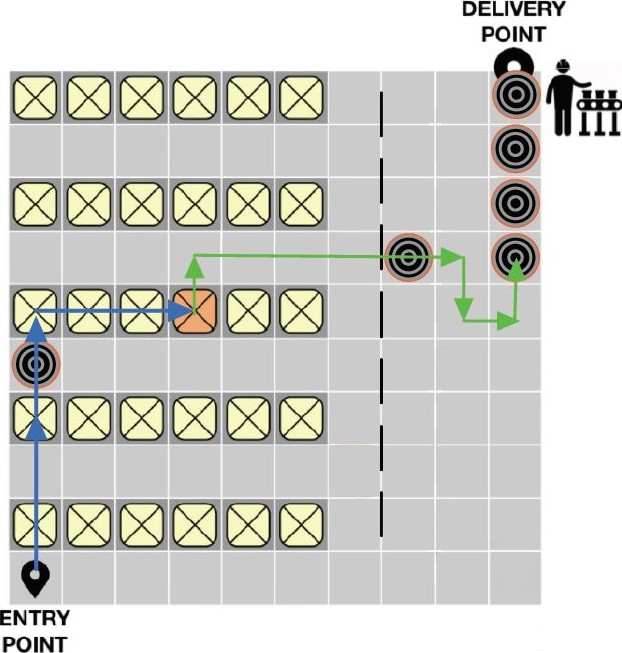
\includegraphics[scale = 0.36]{Images/BotMovement1.JPG}
						\caption{Example of bot movement between entry and delivery point}
					\end{figure}
					\item \emph{From delivery point to pod position} the bot goes right until it reaches the ${(m-2)}^{th}$ column. Then it goes down until it reaches the line before the one it must get in. Here, the bot checks wheter the line is free. If so, it goes to the pod position following a straight path.
					\item \emph{From pod position to the entry point} the bot moves horizontally until it reaches the column corresponding to the entry point. After that, it goes down until it reaches its destination.\footnote{To avoid possible soft locking situations, in case the entry poitn is on the first column, the bot stops its horizontal movement at the second column, then it goes down, and eventually it moves to the right to reach the entry point.}
					\begin{figure}[ht]
						\centering
						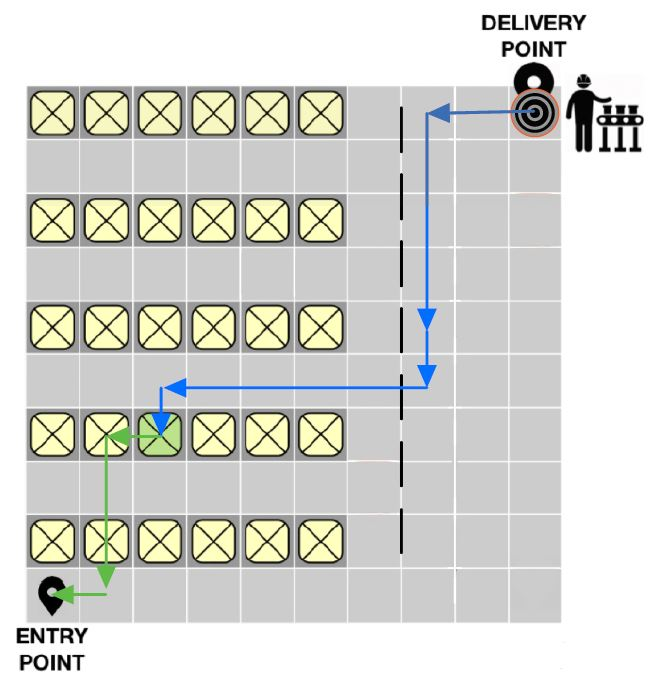
\includegraphics[scale = 0.36]{Images/BotMovement2.JPG}
						\caption{Example of bot movement between delivery and entry point}
					\end{figure}
				\end{itemize}
				\begin{figure}[H]
					\centering
					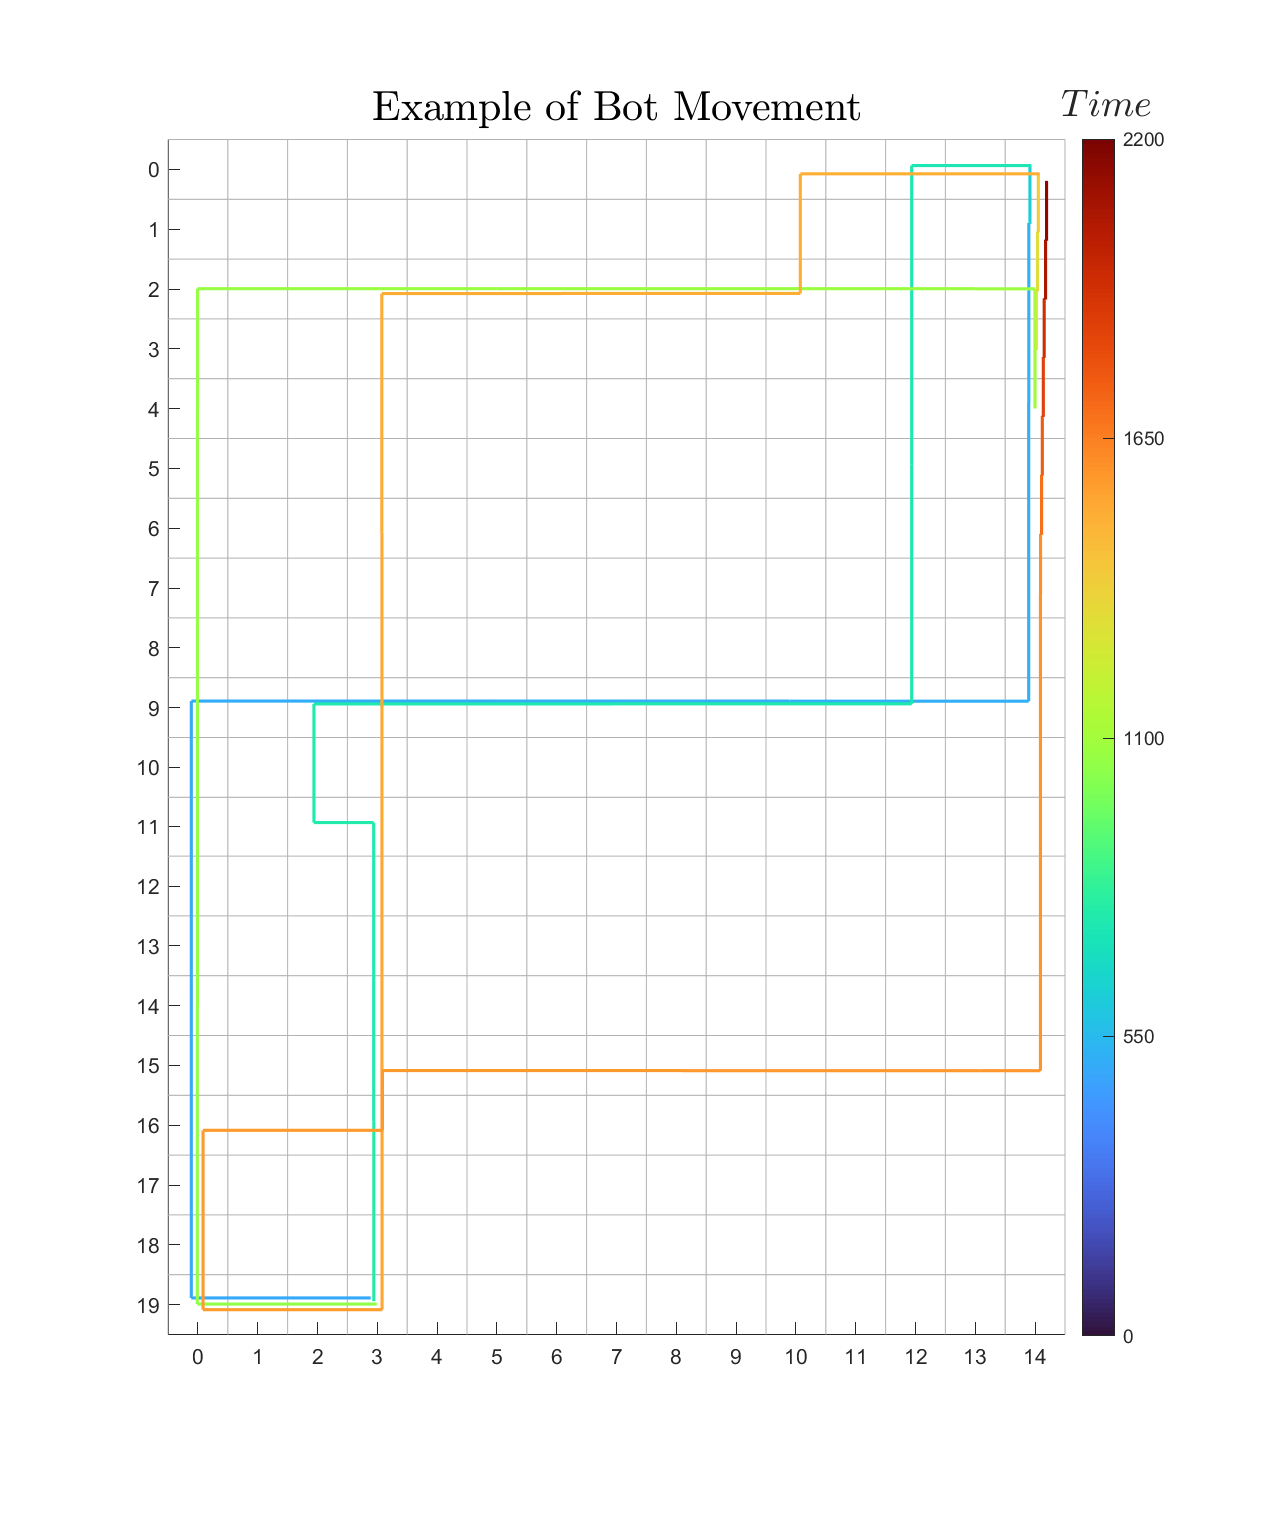
\includegraphics[scale = 0.55]{Images/BotMovement}
					\caption{Example of bot movement with $K=1s$ during a time of $2000s$}
				\end{figure}


		\subsection{Queue}
			The Queue template models the mechanism to manage the arriving of new tasks in the system and their dispatching to the bots. It also carries out the grid initialization.\\
			It is composed of two states:
			\begin{itemize}
				\item An initial \emph{start} state that we made also committed to carry out the queue and grid initializations; originally, the setting of the grid were carried out by a dedicated template, but since it was the only operation in that process we removed it and integrated in this one in order to simplify the model.
				\item A \emph{working} state, that groups the functions of
					\begin{enumerate}
						\item Adding a task to the queue
						\item Removing a task from the queue when it's been claimed by a bot
						\item Keeping count of how many tasks has been issued, how many tasks are executed and how many tasks have been lost
					\end{enumerate}
					This last function is crucial, because the property that must hold in the system throughout the whole test run will directly address the number of tasks that have been lost managed by this process.
			\end{itemize}
			We have initally modeled this template with a state dedicated to each one of the function listed above, then we progressively removed the states "embedding" their functionalities in the transitions and grouping them together. This was done in order to reduce the number of states to verify and improve the verification time. 
		
		\subsection{Task and Human}
			The Task template models the generation process of new tasks. Its parameters sets the values of mean and standard deviation of the normal distribution associated to the "spawn rate" of new tasks.\\
			It's composed of two states:
			\begin{itemize}
				\item A \emph{startingTask} initial commit state that is in charge of initializing the additional data structures of the model, such as the list of available pods.
				\item An \emph{idle} state that just sends tokens on the channel \emph{newTask} at random interval of time (according to the distribution specified).
			\end{itemize}
			\begin{figure}[H]
				\centering
				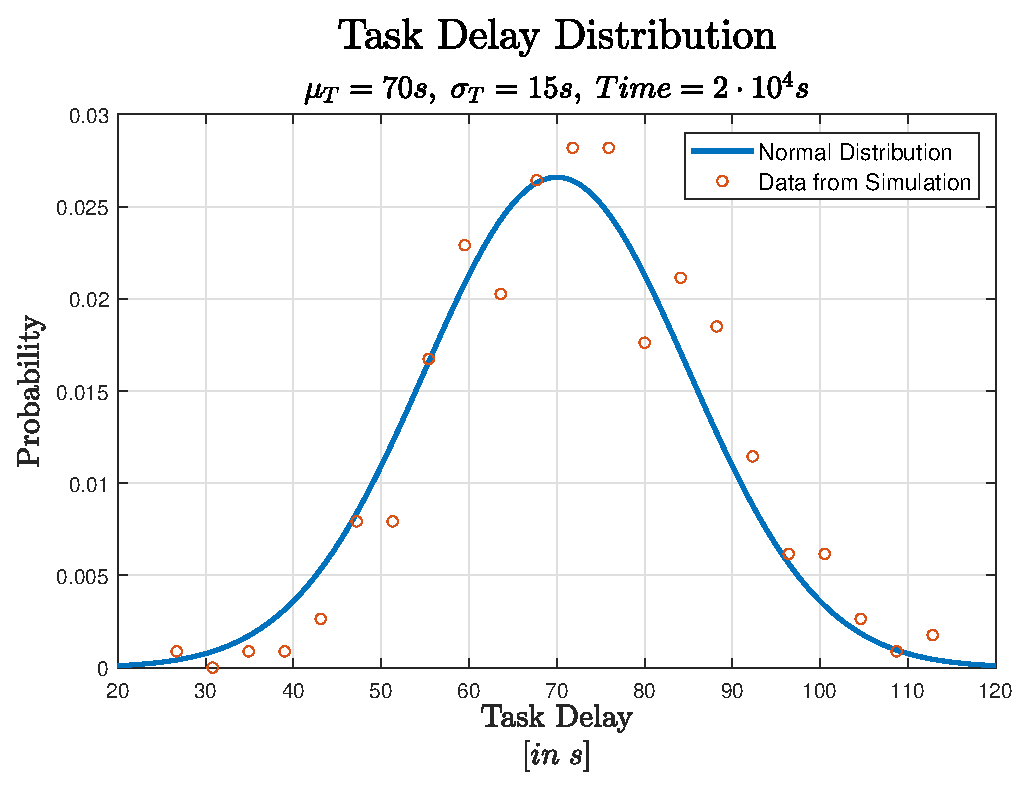
\includegraphics[scale = 0.65]{Images/taskDelay}
				\caption{Example of task delay distribution}
			\end{figure}
			The Human template, instead, models the time elapsed between the robot arrival and departure form the delivery point. Its parameters sets the values of mean and standard deviation of the normal distribution associated to the time needed to complete the job.\\
			It is composed of a \emph{free} state and a \emph{busy} state to model the two possible condition of the human operator. 
			
			\begin{figure}[H]
				\centering
				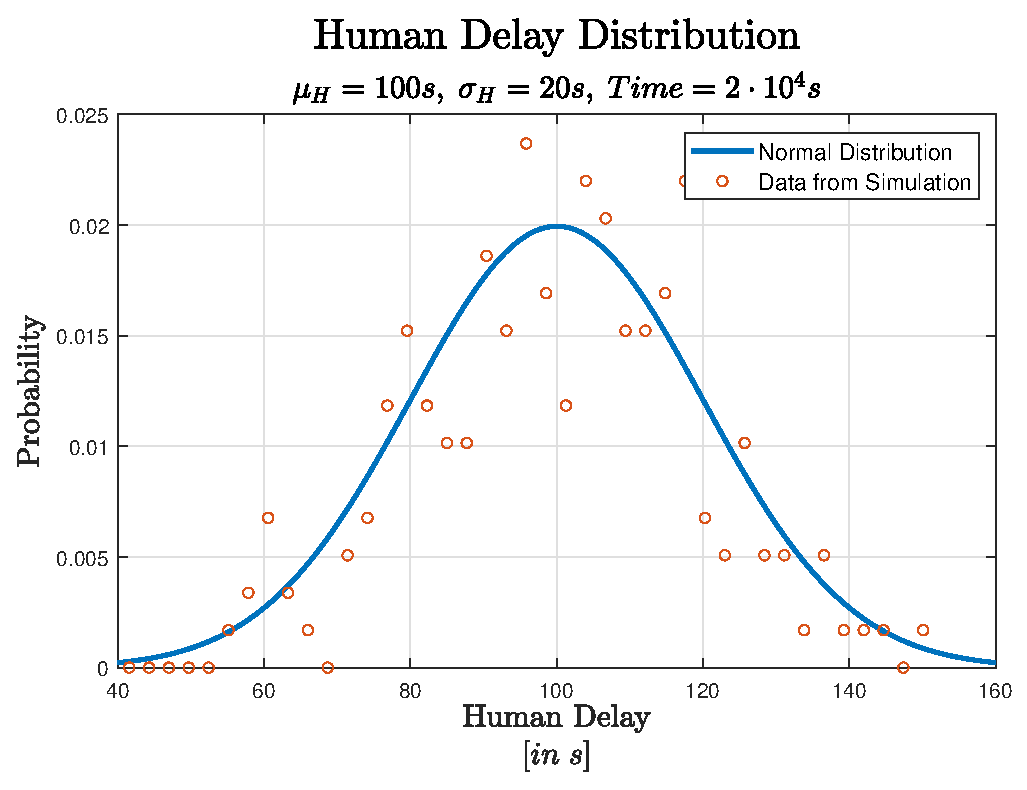
\includegraphics[scale = 0.65]{Images/humanDelay}
				\caption{Example of human delay distribution}
			\end{figure}
	\section{System Configurations}
		We have prepared 4 configurations for the test, the first one that actually fails in proving the searched property in the confidence interval we defined, and the other ones that try to fix the model changing every time a key parameter. In particular, we will try changing the human responsiveness, the number of bots and the time between two tasks.\\
		These parameters do not change among the various configurations:
		\begin{center}
				\begin{tabular}{ |c|c|c|}
					\hline
					Parameter & Value & Additional notes\\
					\hline
					\hline
					Grid width & 15 &\\
					\hline
					Grid height & 20 &\\
					\hline
					Number of pods per row & 11 &\\
					\hline
					Space between rows & 1 &\\
					\hline
					Entry point position & (19, 3) &\\
					\hline
					Delivery point position & (0, 14) &\\
					\hline
					Maximumm queue length & 3 &\\
					\hline
					Robot movement speed & 2 &\\
					\hline
					Robot exponential parameter $\lambda_{bot}$ & 10 &\\
					\hline
				\end{tabular}
			\end{center}
			\begin{figure}[H]
				\centering
					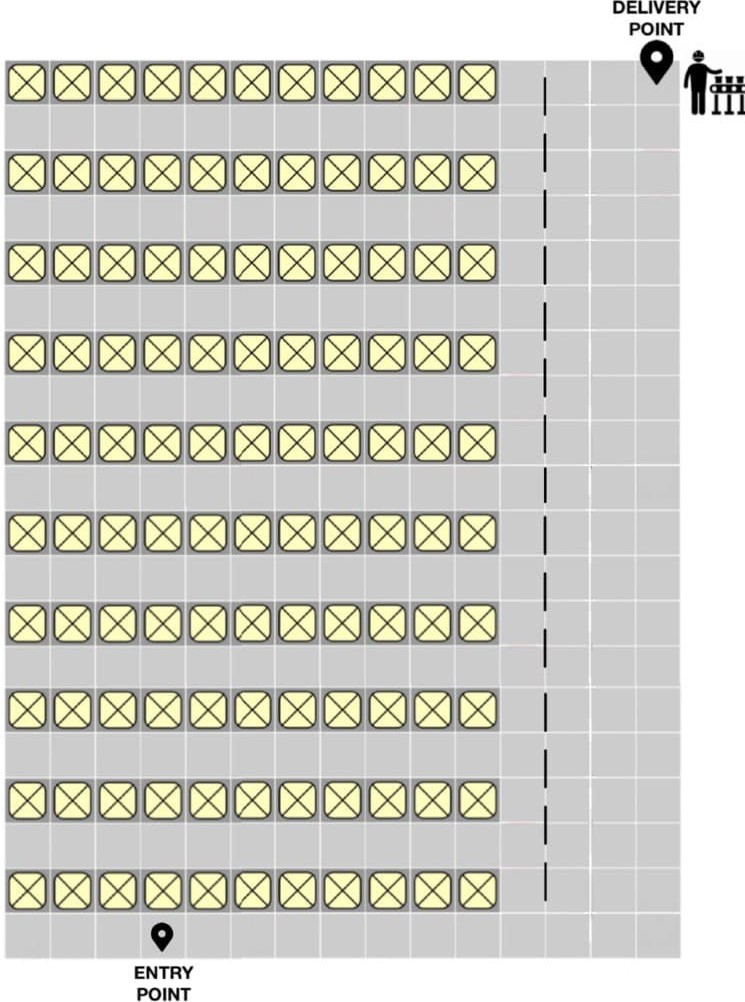
\includegraphics[scale = 0.34]{Images/Grid.jpg}
					\caption{Grid used for simulation}
			\end{figure}

		
		
		\subsection{First Configuration - Failing}
			\begin{center}
				\begin{tabular}{ |c|c|c|}
					\hline
					Parameter & Value & Additional notes\\
					\hline
					\hline
					Number of bots & 8 &\\
					\hline
					Task spawn rate - expected value $\mu_t$ & 70 &\\
					\hline					
					Task spawn rate - standard deviation $\sigma_t$ & 15 &\\
					\hline
					Human response time - expected value $\mu_H$ & 100 &\\
					\hline					
					Human response time - standard deviation $\sigma_H$ & 20 &\\
					\hline
				\end{tabular}
			\end{center}
			\begin{figure}[H]
				\centering
					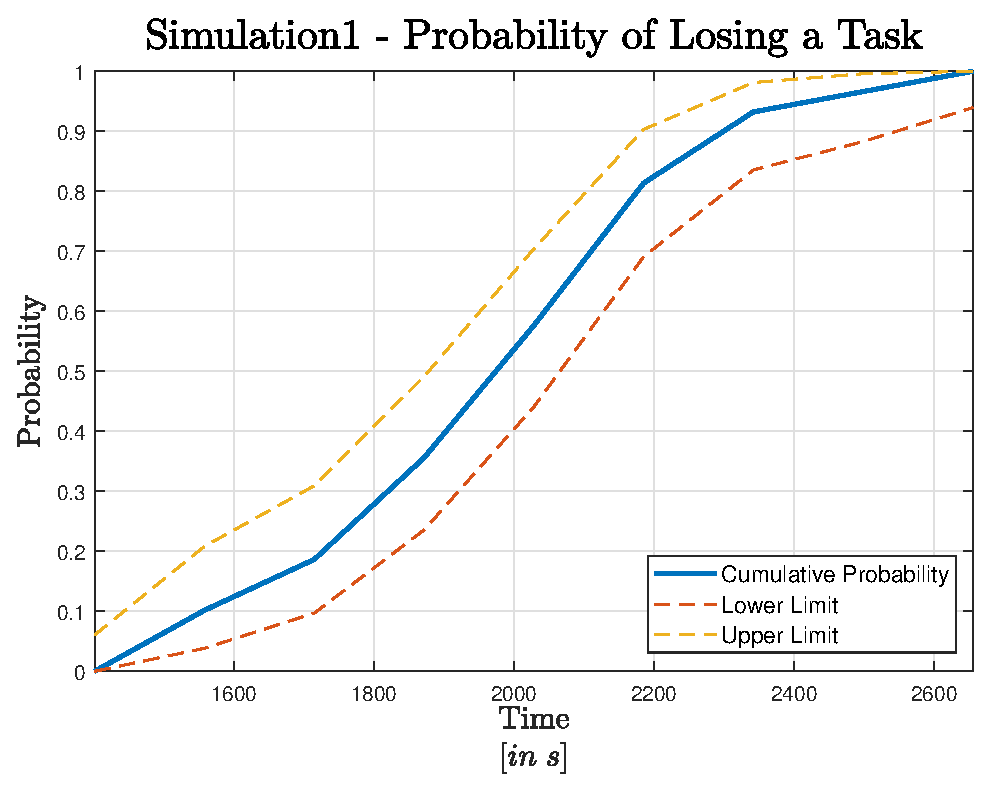
\includegraphics[scale = 0.7]{Images/Simulation1}
					\caption{Probability that a task is lost during simulation 1}
			\end{figure}
		
		\subsection{Second Configuration - Successful}
			\begin{center}
				\begin{tabular}{ |c|c|c|}
					\hline
					Parameter & Value & Additional notes\\
					\hline
					\hline
					Number of bots & 8 &\\
					\hline
					Task spawn rate - expected value $\mu_t$ & 70 &\\
					\hline					
					Task spawn rate - standard deviation $\sigma_t$ & 15 &\\
					\hline
					Human response time - expected value $\mu_H$ & \textbf{60}\footnotemark &\\
					\hline					
					Human response time - standard deviation $\sigma_H$ & \textbf{5} &\\
					\hline
				\end{tabular}
			\end{center}
			\footnotetext{Bold numbers represent parameter changed with respect to the first configuration}	
			
		\subsection{Third Configuration - Failing}
			\begin{center}
				\begin{tabular}{ |c|c|c|}
					\hline
					Parameter & Value & Additional notes\\
					\hline
					\hline
					Number of bots & \textbf{12} &\\
					\hline
					Task spawn rate - expected value $\mu_t$ & 70 &\\
					\hline					
					Task spawn rate - standard deviation $\sigma_t$ & 5 &\\
					\hline
					Human response time - expected value $\mu_H$ & 100 &\\
					\hline					
					Human response time - standard deviation $\sigma_H$ & 20 &\\
					\hline
				\end{tabular}
			\end{center}
			\begin{figure}[H]
				\centering
					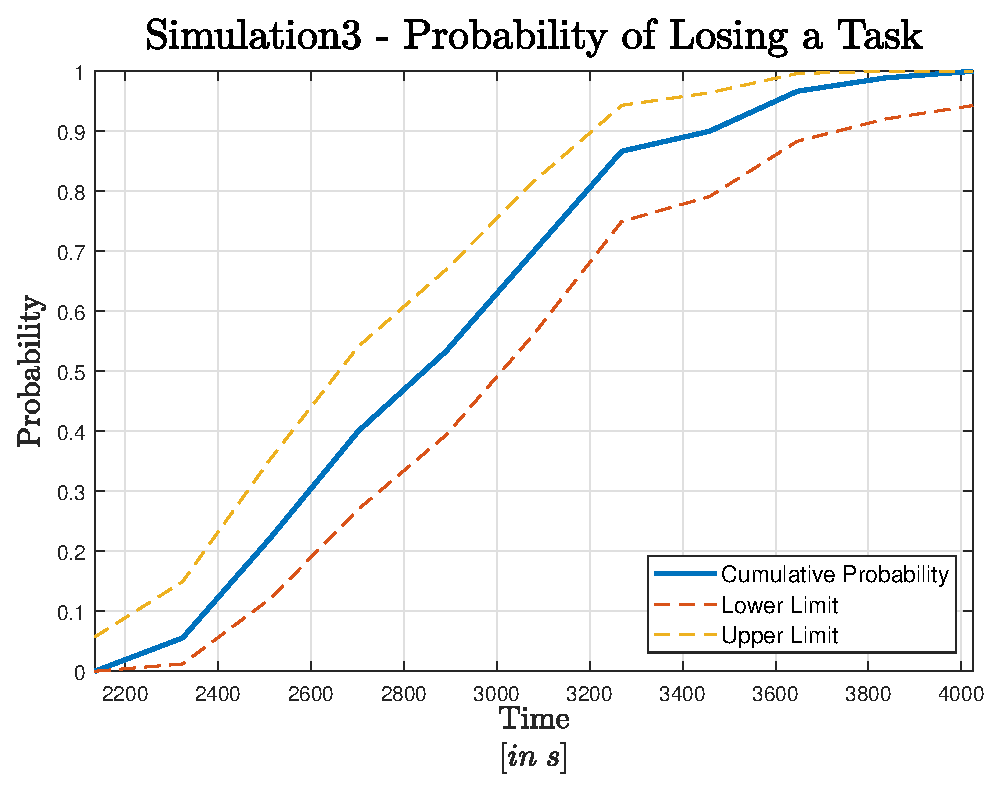
\includegraphics[scale = 0.7]{Images/Simulation3}
					\caption{Probability that a task is lost during simulation 3}
			\end{figure}


		\subsection{Fourth Configuration - Possible Failure}
			\begin{center}
				\begin{tabular}{ |c|c|c|}
					\hline
					Parameter & Value & Additional notes\\
					\hline
					\hline
					Number of bots & 8 &\\
					\hline
					Task spawn rate - expected value $\mu_t$ & \textbf{85} &\\
					\hline					
					Task spawn rate - standard deviation $\sigma_t$ & \textbf{10} &\\
					\hline
					Human response time - expected value $\mu_H$ & 100 &\\
					\hline					
					Human response time - standard deviation $\sigma_H$ & 20 &\\
					\hline
				\end{tabular}
			\end{center}
	
	\section{Experimental Results}
	
	\section{Further Improvement and Alternative Approaches} % sì lo so non ho scritto un cazzo, domani (giovedì) finisco per bene tutto @Simone
		We added this section in order to quickly describe the techniques we used to enhance the \emph{original} non stochastic formulation of the model, because most of them could have been further exploited in a non statistical system.
		
		\paragraph{Variable Reduction}
			While this can seem like a normal practice to model, minimizing the number of the variables and reducing the variables "activity interval"\footnote{a variable v is called inactive in a location l, if along all paths starting from l, v will be reset before it will be used.} is fundamental to reduce the overall number of states that must be checked by the verifier, speeding up verification.
			
		\paragraph{Synchronous Value Passing}
		
		\paragraph{Select Statements Reduction}
		
		\paragraph{Symmetry Reduction}
		
		\paragraph{Sweep Line}
		
	
\end{document}
